\section{Code FLow}\label{sec:c3s3}
	
	\paragraph{}
	A small summary for the flow of the code is given below, and simplified flow chart is in figure ~\ref{fig:simplified_code_flow}:
		
		\begin{enumerate}
			\item The input is an \ac{epr} (counter) satisfiable problem.
			\item Simplified Range Restricted Transformations got applied on the input.
			\item The intermediate output from the transformations act as input for the normal proof procedure.
			\item The output from the prover, which is the saturated set of clauses, is the input for the Bachmair and Ganzinger Model Construction Technique. 
			\item Then the final output is the positive literals of the explicit Model for the given problem.  
		\end{enumerate}
		
		
		\begin{figure}[H]
			\centering
			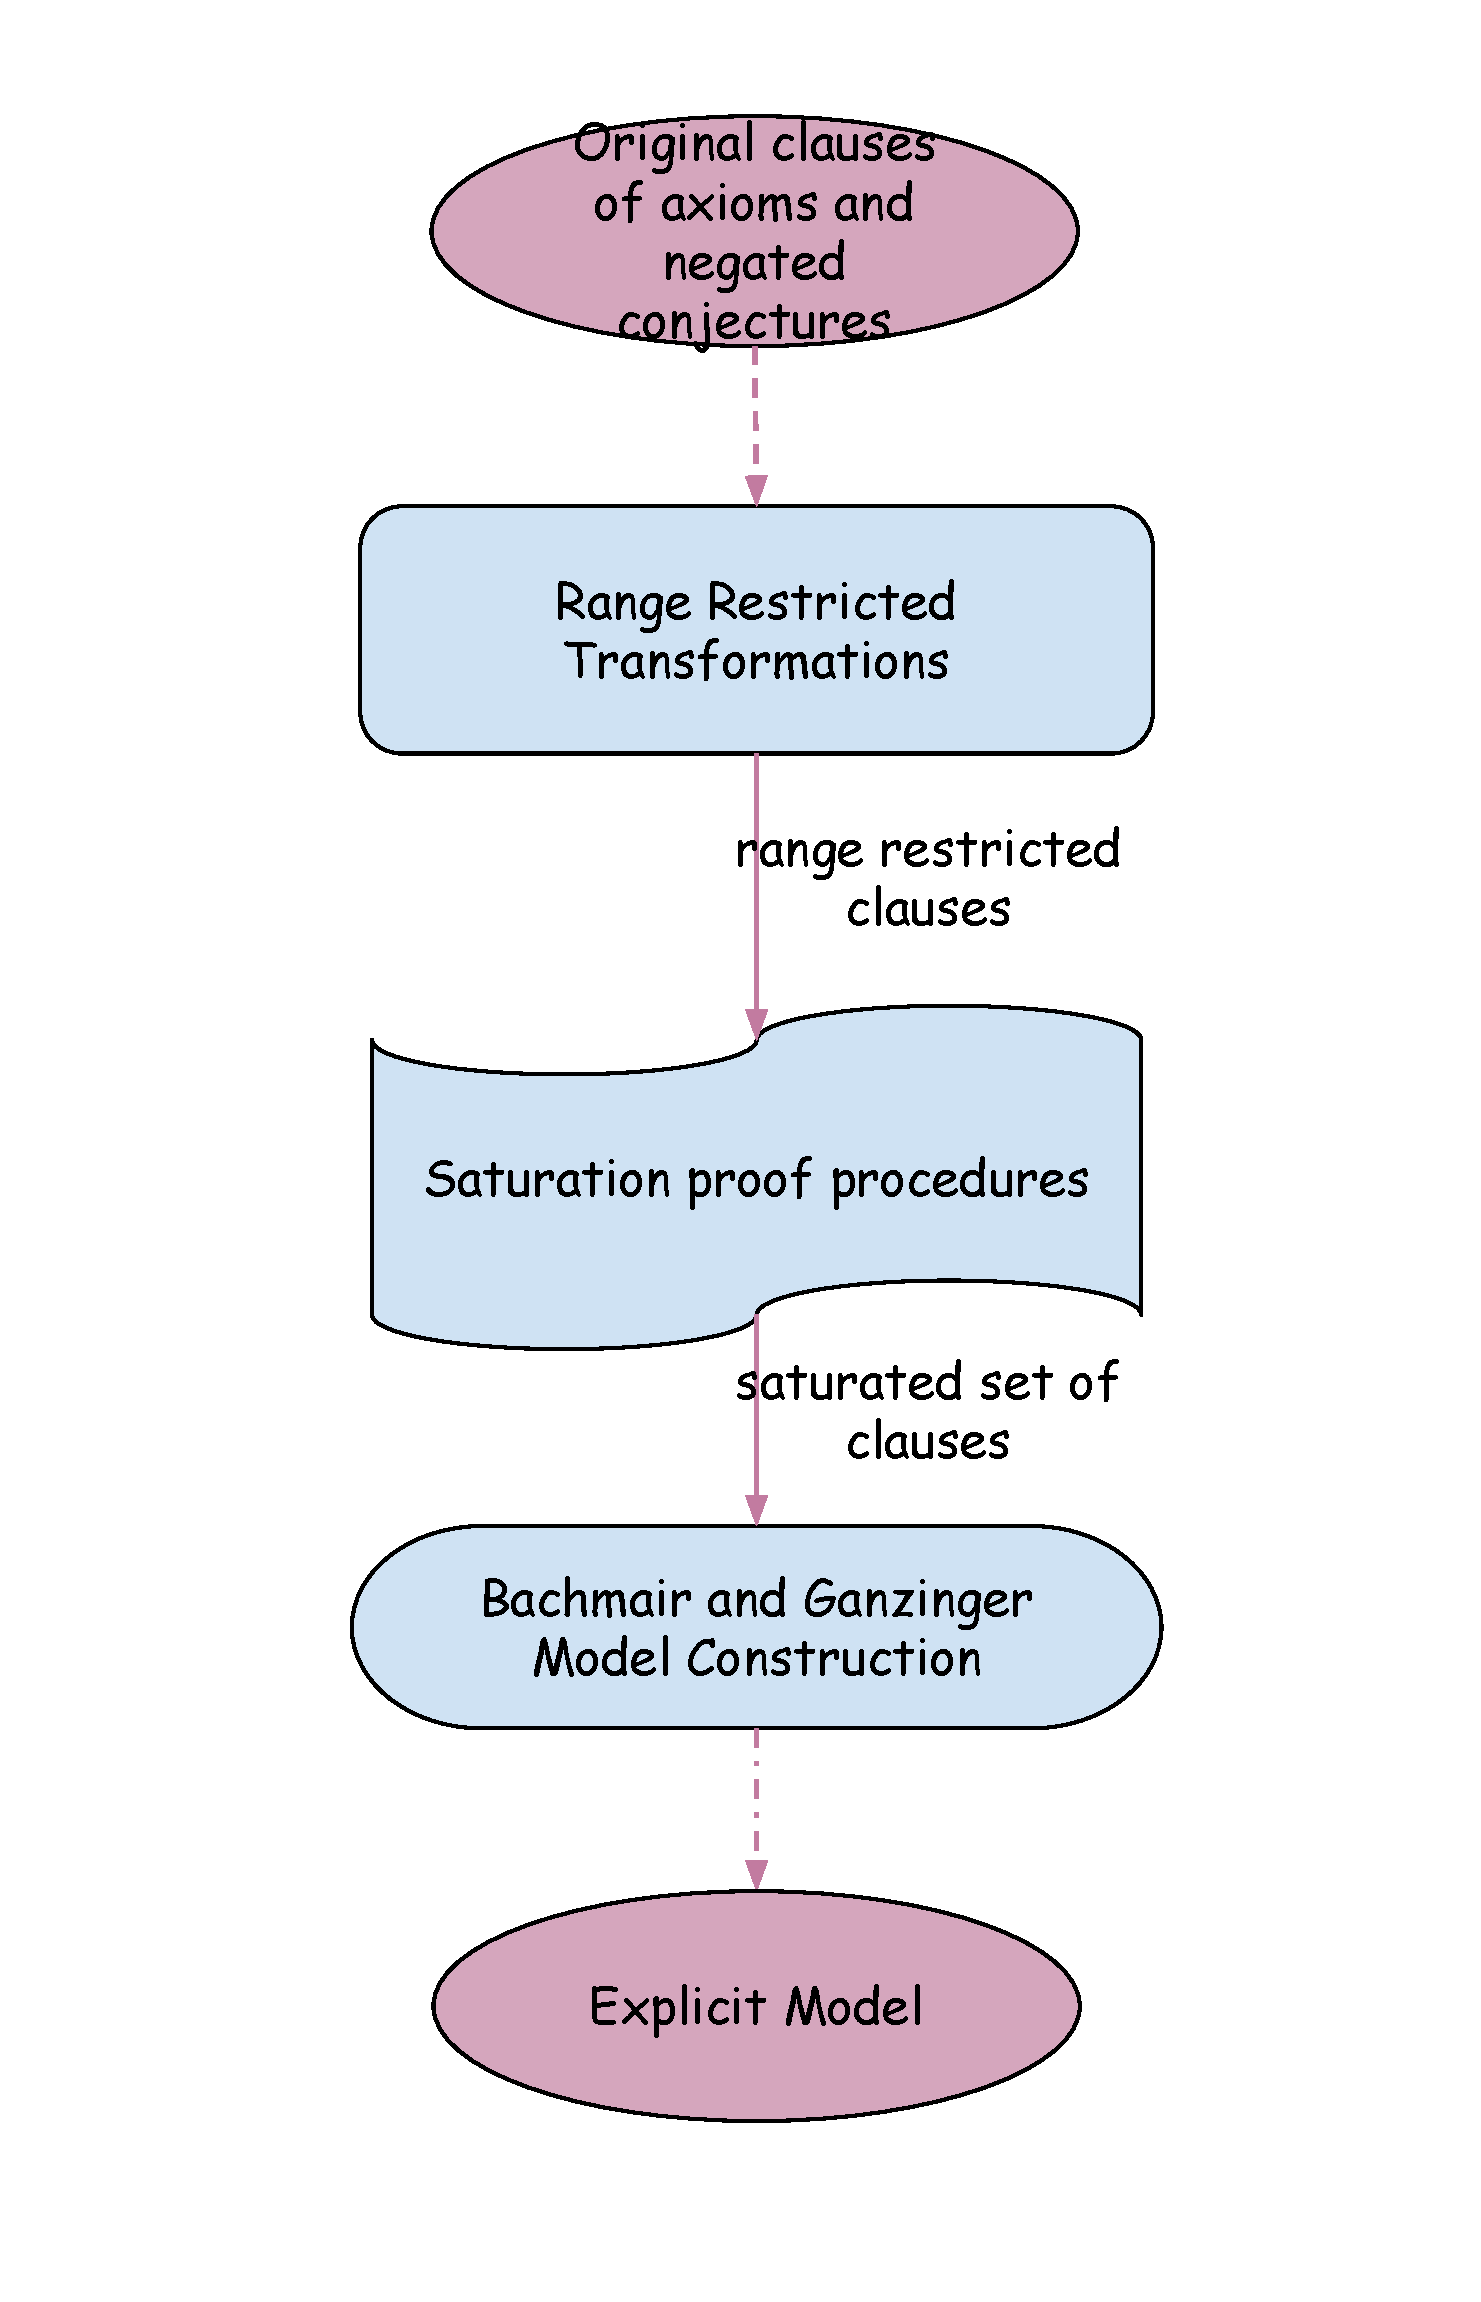
\includegraphics[scale=0.42]{pictures/simplified_code_flow.pdf}
			\caption{Simplified Flow chart for the code flow\label{fig:simplified_code_flow}}
		\end{figure}
		
	